\documentclass[%
	11pt,
	a4paper,
	utf8,
	%twocolumn
		]{article}	

\usepackage{style_packages/podvoyskiy_article_extended}


\begin{document}
\title{Сборник заметок}

\author{\itshape Подвойская Виктория}

\date{}
\maketitle

\thispagestyle{fancy}

\tableofcontents

\listoffigures

\section{СВЧ-разъемы}

Тип соединителя - это конструкция соединителя, которая точно определена для механической и электрической совместимости, а так же для обеспечения повторяемости соединения. Распространенные типы соединителей: тип IX вар. 3, тип III, тип I, тип 3,5 мм, тип N, тип 2,4 мм. Каждый тип соединителя имеет специфические размеры и допуски, связанные с сечением коаксиального тракта. \href{https://www.micran.ru/productions/Accessory/connectors}{Подробнее о СВЧ-разъемах}

Сечение коаксиального тракта – это соотношение диаметров проводников коаксиальной линии передачи. Широко распространены следующие сечения коаксиальных трактов: 2,4/1,042 мм; 2,92/1,27 мм; 3,5/1,52 мм; 7,0/3,04 мм.

Все соединители имеют центральный проводник (ЦП) и внешний проводник (ВП). Центральные проводники бывают с гнездовыми или штыревыми контактами. Как правило, внешние проводники – это корпусы соединителей. У соединителей есть опорная плоскость (ОП) – это плоскость контакта внешних проводников этих соединителей. На рис. 1 показаны ЦП, ВП, ОП и диаметры тракта соединителей вилка и розетка тип 3,5 мм.

В зависимости от области применения, требований к электрическим и механическим параметрам выделяют 3 класса коаксиальных соединителей: общего применения, приборные и метрологические.

Механическая совместимость соединителей. В связи с широким использованием в нашей стране зарубежной СВЧ-аппаратуры существует проблема соединения отечественной и импортной аппаратуры, работающей в одном коаксиальном тракте. Отличие отечественных соединителей от зарубежных аналогов заключается в использовании различных типов резьбы в элементах соединения ВП и в различных диаметрах контактов ЦП.

\begin{figure}[h]
	\centering
	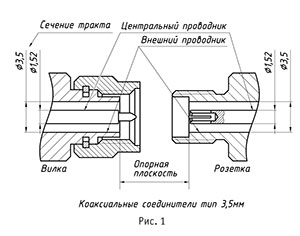
\includegraphics[scale=0.8]{figures/type_3.5.jpg}
	\caption{Коаксиальные соединители}\label{fig:type3_5}
\end{figure}

Проблема совместимости резьбы заключается в том, что, например, внешний диаметр метрической резьбы M6x0,75 равен 6 мм, а у дюймовой резьбы 1/4''-36UNS равен 6,35 мм, поэтому метрический соединитель «вилка» невозможно накрутить на дюймовый соединитель «розетка». Подобная ситуация возникает с резьбами M16x1 и 5/8''-24UENF: внешний диаметр резьбы M16x1 равен 16 мм, а внешний диаметр резьбы 5/8''-24UENF равен 15,87 мм, поэтому дюймовый соединитель «вилка» невозможно накрутить на метрический соединитель «розетка». Однако существует возможность соединить метрический и дюймовый соединители в следующих комбинациях: тип N розетка с типом III вилка; тип SMA вилка и тип 3,5 вилка с типом IX (варианты 1 и 3) розетка; тип K вилка с типом IX (варианты 1 и 3) розетка. Дополнительно при этом необходимо учитывать разницу в шаге резьб. Эта разница не заметна (не происходит заклинивания) при условии, что длины резьб не превышают 3 – 4 витка. При таких соединениях не будет качественного электрического контакта ВП и может произойти механическое повреждение контактов ЦП. Категорически не рекомендуется соединять в таких комбинациях устройства с соединителями приборного и метрологического класса. В табл.1. приведены аналоги зарубежных и отечественных соединителей. Различие диаметров контактов ЦП показано в таблице.

\begin{figure}[h]
	\centering
	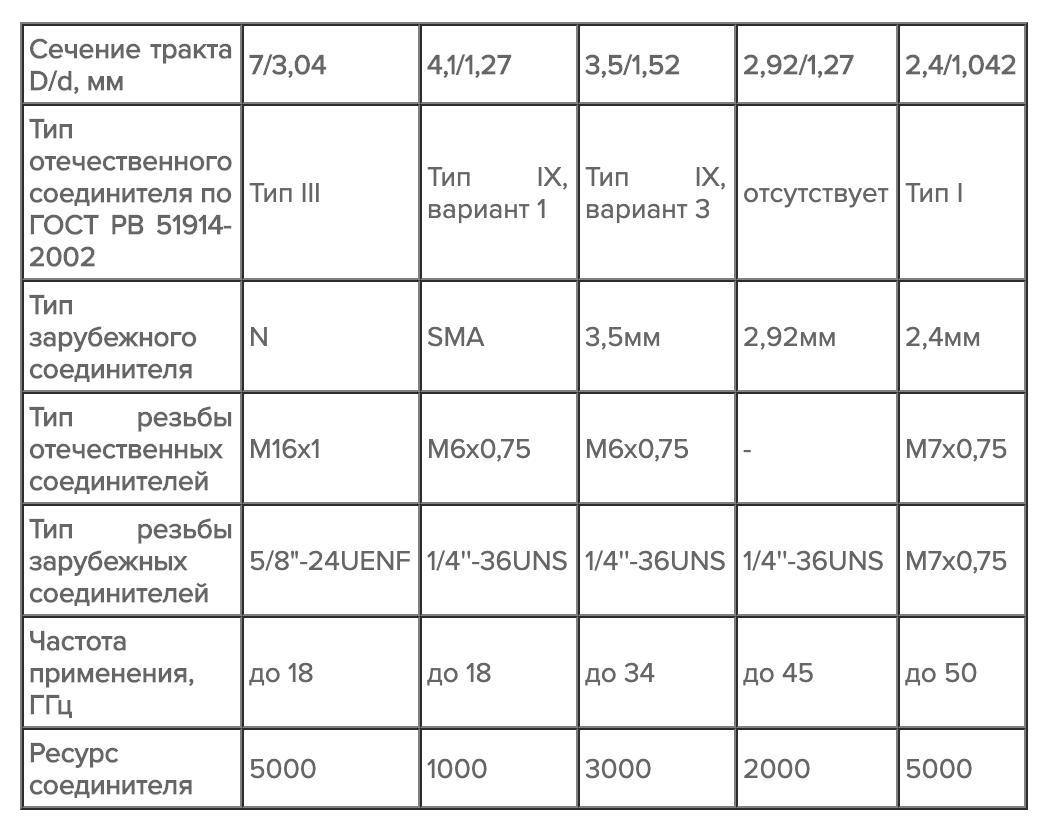
\includegraphics[scale=0.5]{figures/SVCH_table_1.png}
	\caption{Таблица 1}\label{fig:SVCH_table_1}
\end{figure}

Разница диаметров может показаться несущественной, но если не учесть это различие, то можно вывести из строя соединитель, установленный на дорогом оборудовании. При подключении не соответствующих друг другу контактов происходит соединение с повышенными усилиями включения и выключения, что может привести к преждевременному стиранию покрытия штыревого контакта, к поломке ламелей гнездовых контактов, к смещению центральных проводников вдоль оси и к повреждению диэлектрических опор. Как видно из таблицы 2, диаметры отверстий в гнездовых контактах четко не регламентируется. Для гнездовых контактов каждого типа соединителей определено максимальное усилие включения F вкл. max, максимальное усилие выключения F выкл. max (табл. 3), эти параметры заданы для предотвращения указанных выше поломок. Для обеспечения качественного контакта, для гнездовых контактов каждого типа соединителей определено минимальное усилие выключения F выкл. min (табл. 3)

\begin{figure}[h]
	\centering
	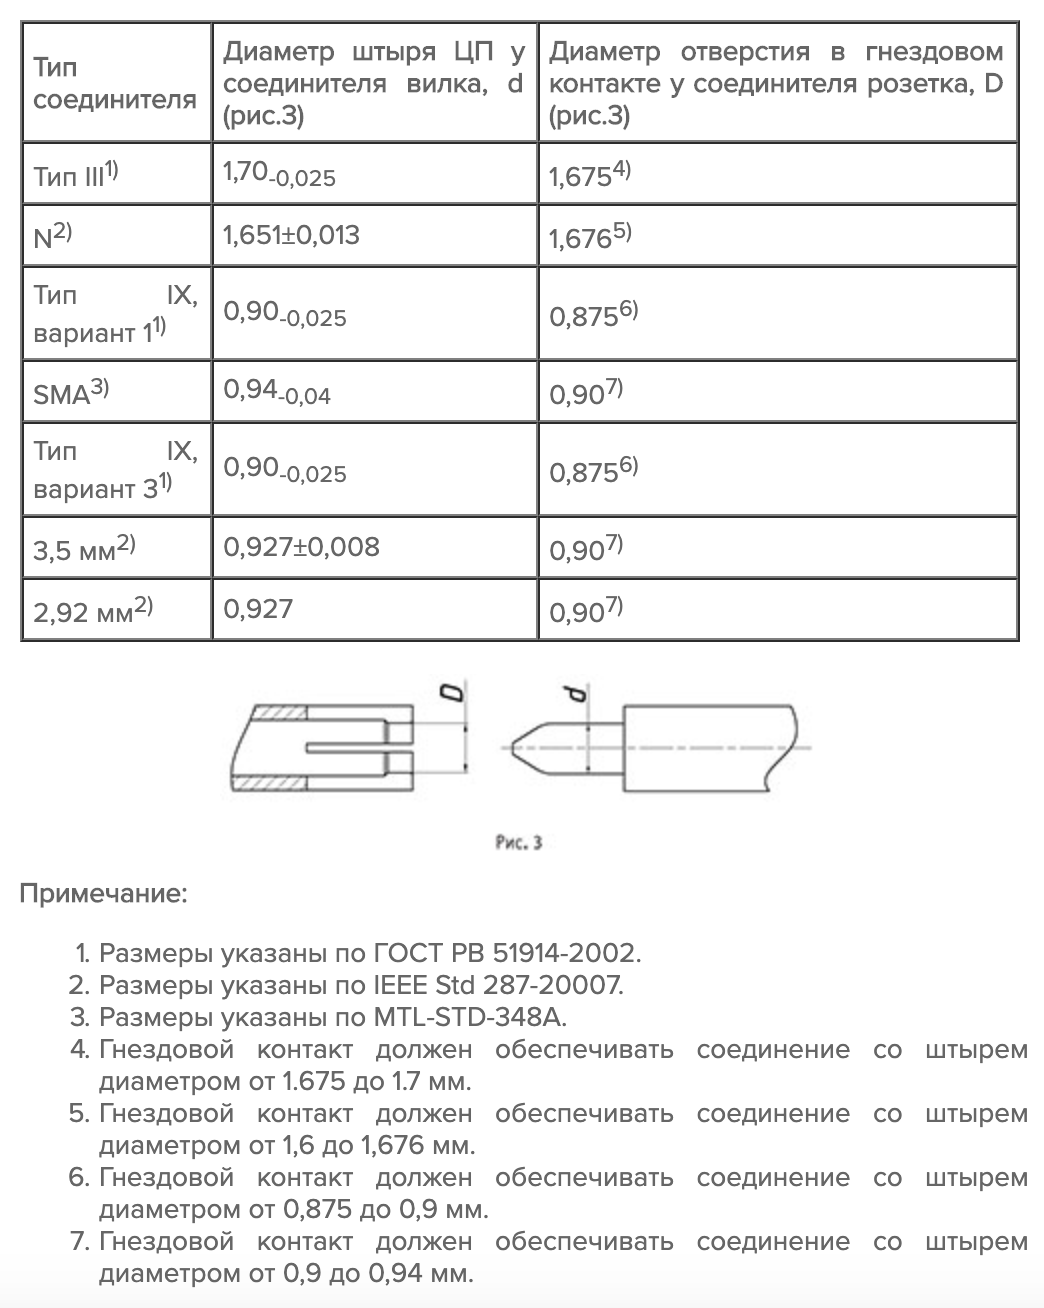
\includegraphics[scale=0.5]{figures/SVCH_table_2.png}
	\caption{Таблица 2}\label{fig:SVCH_table_2}
\end{figure}

\textit{В измерительной технике СВЧ применяются соединители только с воздушным заполнением тракта, такие как тип 2,4 мм, тип 2,92 мм, тип 3,5 мм, тип N, тип I, тип IX вар. 3, тип III.}

\subsection{TNC}
Разъем TNC используется во многих областях, где для обеспечения надежного сопряжения требуется соединитель среднего размера. В общем виде он очень похож на популярный разъем BNC, но, вместо байонетного, он использует резьбовое соединение. Обычно разъем TNC используется там, где разъем должен выдерживать вибрацию и обеспечивать надежную работу на высоких частотах, а удобство байонетного соединения не требуется. Большинство разъемов TNC рассчитаны на 11 ГГц, а некоторые (от известных поставщиков) способны работать на 18 ГГц.
\remark{%
ОСНОВНЫЕ ТЕХНИЧЕСКИЕ ХАРАКТЕРИСТИКИ TNC

Тип кабеля - коаксиальный;

Крепление - резьбовое;

Диапазон рабочих частот - 0 - 11 ГГц;

Диаметр (папа) - 0,590 дюйма (15,0 мм);

Диаметр (мама) - 0,378 дюйма (9,6 мм);

Резьба - 7/16-28 UNEF.
}
TNC с обратной полярностью (RP-TNC, иногда RTNC) является разновидностью разъёма TNC, в которой изменена «половая принадлежность» :) Выпускались они с целью не допустить незаконное использование радиоаппаратуры, например антенн для усиления сигнала Wi-Fi, что противозаконно в некоторых местах.
Вся остальная информация по этому типу разъёмов: виды, методы сборки, наличие переходников и т.д идентична разъёму BNC.

\subsection{N-tipe}
Разъем N-типа - это радиочастотный разъем, используемый там, где требуются высокая мощность, высокие частоты (до 11 ГГц и более) и высокие эксплуатационные параметры.
РЧ разъем N-типа используется во многих приборах, особенно там, где радиочастотные характеристики имеют первостепенное значение.

Разъем N-типа особенно хорош там, где необходимы высокая мощность. Имея б\'{\itshape o}льшие размеры, чем разъемы других типов, например BNC, разъем N-типа подходит для использования с более крупными кабелями с низкими потерями.

Разработка разъема N-типа возникла из-за необходимости в высокопроизводительном радиочастотном разъеме с постоянным импедансом, и его первоначальная цель заключалась в том, чтобы работать на частоте до 1 ГГц. Со времени своего первого внедрения он нашел множество применений в областях, где требуются хорошие ВЧ-характеристики, а также способность передавать высокие уровни мощности и использоваться с коаксиальными кабелями большего размера. Также было показано, что его работоспособность выходит далеко за рамки первоначальной цели 1 ГГц. Разъем имеет резьбовое соединение для обеспечения правильного сопряжения и хорошей работы. Доступны две версии разъема N-типа: 50 Ом и 75 Ом.
Из двух доступных версий этого радиочастотного разъема наиболее широко используется 50-омный разъем N-типа. Это объясняется тем, что в настоящее время системы на 75 Ом редко используются в коммерческих и профессиональных системах связи. Две этих версии разъема N-типа имеют небольшие механические различия, которые не позволяют соединить два типа разъёмов. Если разъёмы двух разных типов соединить, это может привести к их повреждению. Вариант 50 Ом имеет центральный контакт большего диаметра.

Разъем способен выдерживать относительно высокую мощность по сравнению с разъемами BNC или TNC. Стандартные версии предназначены для работы на частотах до 11 ГГц, хотя доступны специальные версии для работы на частотах до 18 ГГц.

Рекомендуемый момент затяжки на наружной оболочке корпуса у разных производителей различен. Зачастую это просто хорошая ручная затяжка, но для более точной информации следует обратиться к паспорту производителя. Как правило, это значение около 1,7 Нм.

\remark{%
ТЕХНИЧЕСКИЕ ХАРАКТЕРИСТИКИ РАЗЪЕМА N-ТИПА

Тип кабеля - Коаксиальный;

Импеданс - 50 Ом и 75 Ом;

Диапазон частот - Обычно 11 ГГц, хотя в некоторых прецизионных версиях указана частота 18 ГГц;

Типичный наружный диаметр (наружный диаметр) - 0,800 дюйма/20,3 мм;

Типичный наружный диаметр (внутренний) - 0,620 дюйма/15,7 мм;

Резьба соединителя - 5/8 дюймов 24 оборота на дюйм. Резьба UNEF.
}

\subsection{BNC}

Это миниатюрные ВЧ-коннекторы с быстрым соединением-разъединением. Они имеют два байонетных выступа на гнездовой части разъема; сочленение
выполняется вращением на четверть оборота сцепляющей гайки. Разъемы идеально подходят
для миниатюрных и субминиатюрных кабелей (типов -58, 59, … , -179, -316 и т.д.).
Выпускаются в соответствии со стандартами и
50-омные предназначены для работы на частотах до 11 ГГц и обычно имеют низкое
отражение до 4ГГц. 75-омных -коннекторы отличаются постоянством импеданса с низким
КСВН до 4 ГГц. Эти соединители могут использоваться в самых разнообразных вариантах, где
необходимо обеспечить малое искажение сигнала как в медицинской и
измерительной аппаратуре.

\subsection{SMA}

Данные коннекторы предусматривают использование при параметрах проводника 18 ГГц и 50 Ом. А некоторые прецизионные модели могут функционировать при частоте до 26,5 ГГц. Резьбовое соединение sma-разъема1/4-36 отличается малыми габаритами и прекрасной механической долговечностью. Причем максимальные значения используемых рабочих частот зависят исключительно от типа используемого кабеля.

Коннекторы делятся по способу соединения на устройства с байонетным, врубным и резьбовым соединениями. А по виду монтажа они разделяются на три вида: паяные, обжимные и накручивающиеся. Кроме того, SMA-разъемы отличаются по своим конструктивным особенностям. Бывают кабельные, приборные, монтируемые на печатную плату и переходники. Соответственно кабель монтируется путем обжима или пайки, приборные устройства устанавливаются на корпус за счет крепления гайкой или квадратным фланцем, монтаж коннекторов на плату осуществляется путем пайки (горизонтальной или вертикальной относительно поверхности монтажа), а переходники используются для монтажа разнотипных соединителей.

Кроме того следует знать, что для частот, превышающих стандартные (до 18 ГГц и до 26,5 ГГц), используются следующие коннекторы аналогичные SMA:

- до 34ГГц – 3,5-мм разъемы;

- до 46 ГГЦ – 2,92-мм разъемы.

Вышеуказанные коннекторы в своей конструкции имеют наружную резьбу и могут соединяться со SMA-разъемами. Однако они используют воздух в качестве диэлектрика, и при соединении со SMA-разъемами низкого качества их срок службы может значительно уменьшиться.

\subsection{QMA}

Соединители QMA появились как альтернатива
традиционным SMA разъемам с возможностью быстрого
соединения. 

Преимущества QMA серии:

- быстрое соединение;

- возможность вращения кабеля после установки;

- большая плотность размещения;

- отсутствие проблем с усилием фиксации;

- габариты масса аналогичные SMA. 

Соединители SMA и QMA имеют одинаковую коаксиальную линию, а значит, и одну и ту же предельную рабочую частоту. Однако применение в соединителях QMA нового механизма соединения розетки и вилки — "snap-lock" (вместо резьбового соединения в SMA) — позволило не только уменьшить размеры, но и в 10 раз сократить время соединения. Для соединения розетки и вилки в полевых условиях требуется менее 2 с.

Механизм соединения состоит из подпружиненного наружного проводника вилки, в котором блокируется ответный наружный проводник розетки со специальным буртиком. Рассоединение происходит при отводе стопорной муфты на корпусе вилки. После соединения возможен поворот кабельной вилки на 360°.

Соединение "snap-lock" сочетает высокий уровень параметров, свойственный резьбовым соединителям, с возможностью простого и быстрого соединения и рассоединения вилки и розетки в соединителях с защелкиванием.

По сравнению с соединителями SMA, соединители QMA обеспечивают бoльшую плотность компоновки изделий, так как не требуют дополнительного места под ключ для соединения и рассоединения розетки и вилки. Расстояние между осями соединителей при установке в ряд — 12,4 мм (для соединителей SMA минимальное расстояние — 14 мм).

Соединители QMA предназначены для применения в мобильных базовых станциях систем телекоммуникации и носимых персональных средствах связи.

Так как у соединителей QMA и SMA разные механизмы соединения, они совместимы между собой только при использовании адаптера. Соединители QMA предназначены для работы в частотном диапазоне DC — 18 ГГЦ, однако оптимальный уровень КСВН они имеют на частотах только до 6 ГГц.



\subsection{SMP}

Разъемы SMP спроектированы для максимальной плотности установки. Их конструкция позволяет устанавливать модули с расстоянием между центрами 4,3 мм. Прочный интерфейс разъема может выдерживать суровые условия, механические удары, вибрации обычно встречающиеся в военных и аэрокосмических приложениях.

За рубежом соединители SMP широкой номенклатуры
выпускают более 30 компаний. В  нашей стране
соединители SMP были разработаны компанией
"НПП  Исток" (г. Фрязино) и  затем воспроизведены
в  ПАО  "Иркутский релейный завод"  – ПАО "ИРЗ".
Кроме того, в НПФ "Микран" (г. Томск) созданы приборная вилка и ответный к ней прямой кабельный соединитель SMP.
Интерфейс соединителей SMP соответствует военному стандарту MIL-STD-348A, а их параметры – стандарту MIL-PRF-39012. Подобно другим соединителям,
законченное соединение состоит из  вилки и  розетки.
Большинство производителей называют вилкой соединитель со  штыревым центральным проводником,
розеткой – с гнездовым проводником, хотя по своему
назначению приборные соединители со штыревым центральным проводником  – это розетки, а  кабельные с гнездовым проводником – вилки. 
Компании-производители представляют соединители
SMP с  волновым сопротивлением 50 Ом как соединители с  предельной частотой 40  ГГц. Однако в  полной
мере это утверждение относится лишь к  адаптерам
bullet и  к  некоторым типам прямых кабельных соединителей. Речь идет лишь о том, что в соединителях SMP
коаксиальная линия, заполненная твердым диэлектриком, эквивалентна воздушной коаксиальной линии
2,92-мм соединителей, имеющих приемлемый уровень КСВн и потерь на частотах до 40 ГГц [1]. Реальные
электрические параметры соединителей SMP зависят
от  многих факторов: типа соединителей (кабельные,
приборные, для установки на платы, прямые или угловые), кабеля и способа его заделки в соединитель, способа установки соединителя в корпус или на плату [1].
Требования к  параметрам соединителей SMP приведены в спецификациях DSСC 94007/08 (Defense Supply
Center, Columbus). Электрические параметры зарубежных соединителей SMP показаны в табл.1 [1].
Номенклатура и  основные параметры отечественных соединителей SMP приведены в табл.2.

К соединителям SMP предъявляются следующие
требования:

•	 максимальное рабочее напряжение 335 В на уровне
моря, 65 В – на высоте 21,3 км;

•	 напряжение пробоя 500  В  на  уровне моря, 125  В  –
на высоте 21,3 км;

•	 минимальное сопротивление изоляции 5000 МОм;

•	 максимальное сопротивление: центрального проводника 6 мОм, наружного проводника – 2 мОм;

•	 диапазон рабочих температур: от –65 до 165 °C;

•	 максимальное усилие сочленения вилки и розетки:
68Н (полное защелкивание), 45Н (ограниченное
защелкивание), 9Н (скользящее соединение);

•	 минимальное усилие расчленения вилки и розетки:
22Н (полное защелкивание), 9Н (ограниченное защелкивание), 2,2Н (скользящее соединение);

•	 допустимое количество циклов сочленение-расчленение: 100 (полное защелкивание), 500 (ограниченное защелкивание), 1000 (скользящее соединение);

•	 допустимое радиальное и  аксиальное смещение между осями вилки и  розетки при сочленении 0,25 мм. \href{https://ecworld.ru/media/bip/pdfs/djurinsky_ntb615.pdf}{Подробнее о SMP-разъемах}

\subsection{MCX, MMCX и MMBX}

MCX разъемы - микроминиатюрные коннекторы, внедренные в 1980-е годы и соответствующие требованиям европейского стандарта CECC 22220. Имеют те же размеры центрального контакта и изолятора , что и SMB коннекторы, но внешний диаметр гнезда составляет 0,14 дюйма, что на 30% меньше, чем у разъемов SMB серии. Эта особенность предоставляет конструкторам возможность использовать их там, где особенно высоки требования к экономии места и веса. Механизм защелкивания обеспечивает возможность быстрого соединения/разъединения. MCX выпускаются с импедансом 50 и 75 Ом и способны работать с низким отражением на частотах до 6 ГГц и 1.5 ГГц, соответственно.

MMCX разъемы (уменьшенный вариант MCX)- называется также С2.5 или MicroMate. Это линейка одних из самых маленьких ВЧ разъемов, разработанных фирмой Амфенол в 1990-е гг. и представляет собой серию микроминиатюрных соединителей с механизмом защелкивания, позволяющим вращение на 360°, что обеспечивает гибкость при использовании с печатными платами. MMCX коннекторы удовлетворяют требованиям европейской спецификации CECC22000. Это семейство устройств представляют собой систему межсоединений с импедансом 50 Ом и обладает широкополосными параметрами с низким отражением до 6 ГГц, обеспечивающими высокое качество передачи сигнала. Выпускаются соединители разного типа: кабельные, для поверхностного монтажа и торцевые (гребенчатые) для печатного монтажа.

Соединители MMBX предназначены для реализации непосредственных соединений между печатными или компактными модулями СВЧ. Конструкция соединителей MMBX позволяет компенсировать значительные осевые и радиальные смещения. Отличительными особенностями MMBX серии являются миниатюрность, экономичность и широкий ассортимент конфигураций.

\section{Виды схем}

 Схема-документ, на котором доказаны в виде условных графических изображений или обозначений составные части изделия и связи между ними (ГОСТ 2.102-68).

Схемы в зависимости от видов элементов, входящих в состав изделия, и связей между ними подразделяют на виды, обозначаемые буквами (ГОСТ 2.701-84):

электрические – Э; пневматические – П; газовые (кроме пневматических) - X; кинематические – К; гидравлические – Г; вакуумные – В; оптические – Л; энергетические – Р; деления - Е; комбинированные – С.

В зависимости от основного назначения схемы подразделяют на тины. Типы схем обозначаются цифрами:

структурная – 1; функциональная – 2; принципиальная – 3; соединений – 4; подключения – 5; общая – 6; расположения – 7; объединения – 0,

например, схема электрическая принципиальная Э3 (шифр схемы).

Элемент схемы – составная часть схемы, которая выполняет определенную функцию в изделии и не может быть разделена на части, имеющие самостоятельное назначение (резистор, транзистор и т.п.).

Общие требования к выполнению схем (ГОСТ 2.701-84)

Каждый вид электрической схемы реализуется в виде чертежа или графического изображения, выполненного вручную или посредством печатных приспособлений. Основные отличия обусловлены описанием тех или иных функций, указанием последовательности, принципа действия или привязкой к чему-либо.

Принцип построения схем регламентируется стандартом ЕСКД, который реализуется рядом нормативных документов, среди которых достаточно важными считаются ГОСТ 2.702-2011, а также ГОСТ 2.708-81.

Они устанавливают:

требования к изображениями;
принципам расположения компонентов;
оформления чертежей;
нанесению обозначений и технических характеристик.

Далее детально рассмотрим особенности каждого вида электрических схем.

\textbf{Принципиальная (полная) (3)}

Принципиальная схема предназначена для пояснения принципа действия того или иного устройства. Наиболее часто ее применяют для различных распределительных устройств в силовых цепях, каких-либо приборов и т.д.

На принципиальных схемах обязательно указываются действующие электрические компоненты и проводимые связи между ними, силовые контакты и электрически узлы, соединяющие радиодетали. В свою очередь, такие электрические схемы подразделяются на два подвида: однолинейные и полные.

Однолинейные также называют первичными цепями, на них, как правило, обозначается силовая часть оборудования или электроустановки. С другой стороны однолинейная схема широко распространена для обозначения трехфазных цепей, где все оборудование на трех фазах имеет идентичное расположение и подключение. За счет чего в однолинейном варианте демонстрируется только одна фаза с  некоторыми отступлениями в местах, где оборудование на разных фазах отличается.

Кроме силовых цепей существуют и слаботочные, для питания защит, средств измерительной техники и различных электронных устройств. Такие схемы вторичных цепей называются полными, так как показывают полную картину всего оборудования, выделяя даже состояние некоторых контактов и частей оборудования. Увы, из-за сложности современной аппаратуры, далеко не все устройства можно изобразить на одном листе, поэтому полные бывают элементными и развернутыми.

\textbf{Структурная (1)}

На структурных схемах осуществляется общее изображение устройства, все компоненты или отдельные узлы которого выполняются в виде блоков, обозначающих оборудование, а связи между блоками могут говорить о тех или иных операциях, связующих отдельные блоки между собой.

Структурная схема
Этот тип графического изображения  призван дать общее представление об устройстве и принципе действия, поэтому на них часто проставлены стрелочки, имеются поясняющие надписи и прочие обозначения, упрощающие понимание процесса или поясняющие работу прибора. Для работы с таким изображением не нужно иметь электротехнического образования, так как ее обозначения будут понятны даже не искушенному в электричестве человеку.


\textbf{Функциональная (2)}

Функциональная схема является более детальным вариантом структурной, на ней также все элементы изображаются отдельными блоками. Главное отличие в том, что каждый блок имеет уже индивидуальную форму обозначения в соответствии с  его функциональным назначением. Возможно также выделение различных видов связей между частями, объединение деталей в блоки и т.д.

\textbf{Общая (6)}

Общая схема предназначена для изображения мест расположения электрических аппаратов на местности или в пределах электроустановки. Определяет основные типы электрических соединений этих аппаратов, места их реализации и т.д. Данный тип является обязательным при разработке различных конструкторских документов на этапе проектирования. Но кроме общей, конструкторская документация включает в себя еще две не менее важные схемы – соединений и подключений.

\textbf{Схема соединений (монтажная) (4)}

Схема соединения используется для графического изображения мест подключения электрооборудования. На ней указываются конкретная привязка к частям зданий, распредустановок, по отношению к которым и должен осуществляться монтаж электрооборудования, благодаря чему такой тип схем еще называют монтажными.

Наиболее часто монтажные схемы используются для обозначения разводки электрических цепей в здании, широко применяются во время ремонта, чтобы обозначить места прокладки проводки, установки распределительных коробок и вывода точек подключения к приборам и контактам аппаратов.

На рисунке выше приведен пример монтажной схемы, как видите, для каждого варианта могут устанавливаться свои условные обозначения, указываемые отдельно. Имеются привязки к каждой конкретной комнате и планируемому электрооборудованию, осветительным приборам и т.д. В дальнейшем она используется не только для монтажных работ, но может применяться и в процессе эксплуатации.


\textbf{Подключений (5)}

Схема подключения используется для указания принципов соединения различных электрических или электронных блоков в единую систему. Иногда предполагается, что блоки имеют территориальное разделение, в других ситуациях они могут находиться в пределах одного распределительного устройства, шинной сборки или стойки. Ее пример  приведен на рисунке ниже:

Схема подключения
В зависимости от сложности графического изображения и количества отображаемых подключений оно может дополняться таблицами соединений для пояснения порядка расположения выводов и подключения изделия.

\textbf{Схема расположения (7)}

Также входит в состав проектной документации и помогает определить местоположения всех частей электроустановки относительно друг друга и других значимых объектов.

На схеме расположения могут наноситься:

составные части всего объекта, а при необходимости и связи между всеми частями;

соединительные провода, кабели, шнуры и т.д. в упрощенном виде;

наименование каждого элемента, его тип и документ, на основании которого он применяется.

Такое изображение может выполняться как в двухмерном, так и в трехмерном пространстве. Но в любом случае изображение должно соблюдать масштаб по отношению к натурным размерам и расстояниям.

\textbf{Объединенная схема (0)}

Объединенная схема строиться на основании нескольких типов изображений, рассмотренных нами ранее. Такое построение призвано упростить работу электромонтажников или проектировщиков за счет объединения различной информации в единое целое. Но на практике далеко не всегда целесообразно объединять несколько типов графических элементов. Это связанно со сложностью некоторых приборов и устройств, в которых из-за нагромождения элементов довольно сложно объединять разные изображения.





\section{Comsol}

\subsection{Вебинары}

\subsubsection{Проведение вибрационного анализа в Comsol Mph}

Расчет перемещений при гармонических нагрузеках - Frequency Domain
Задание стационарной нагрузки - Time Domain (Stationary). Frequency Domain - дает значительный выигрыш по времени (на примере в 40 раз).



\section{Python Django(Skillbox)}

\subsection{Введение в веб-фреймворки}

Веб-приложение формирует ответ для пользователя. Веб-сервер принимает запрос пользователя. Веб-приложение и веб-фреймворк - понятия \textbf{тождественные но не равные}.

HTTP-протокол - гипертекстовый протокол обеспечивающий взаимодействие между клиентом и сервером. Специальное соглашение которое поддерживают все клиенты по всему миру. 

HTTP-запрос состоит из головы и тела запроса. Тело - не обязательный параметр. Первое что указывается в голове - это тип запроса(типов запросов много. Мы рассматриваем только GET и POST). GET для запроса информации с сервера. POST для обновления информации на сервере.

Когда мы пишем приложение, мы пишем код, который обрабатывает запросы. Внутри запроса находятся параметры, которые называются заголовками. Параметр HOST указывает к какому хосту на сервере обращается приложение(так как на одном сервере возможно размещение нескольких приложений). В USER AGENT отображается информация о браузере и ОС пользователя. В ACCEPT указывает формат ответа ожидаемый пользователем. HTTP-протокол не сохраняет состояние данных, т.е. при следующем запросе данные заголовков следует продублировать.

Не всегда ответом сервера на HTTP-запрос является HTML-страница. Числовые значения ответов сервера называеются кодами состояния. Первая из трех чисел - класс состояния.

По умолчанию в Python установлена библиотека http. В ней реализованы 2 класса: HTTPServer и BaseHTTPRequestHandler. HTTPServer обеспучивает логику реализации непосредственно веб-сервера. BaseHTTPRequestHandler позволяет обрабатывать запросы.

\begin{figure}[h]
	\centering
	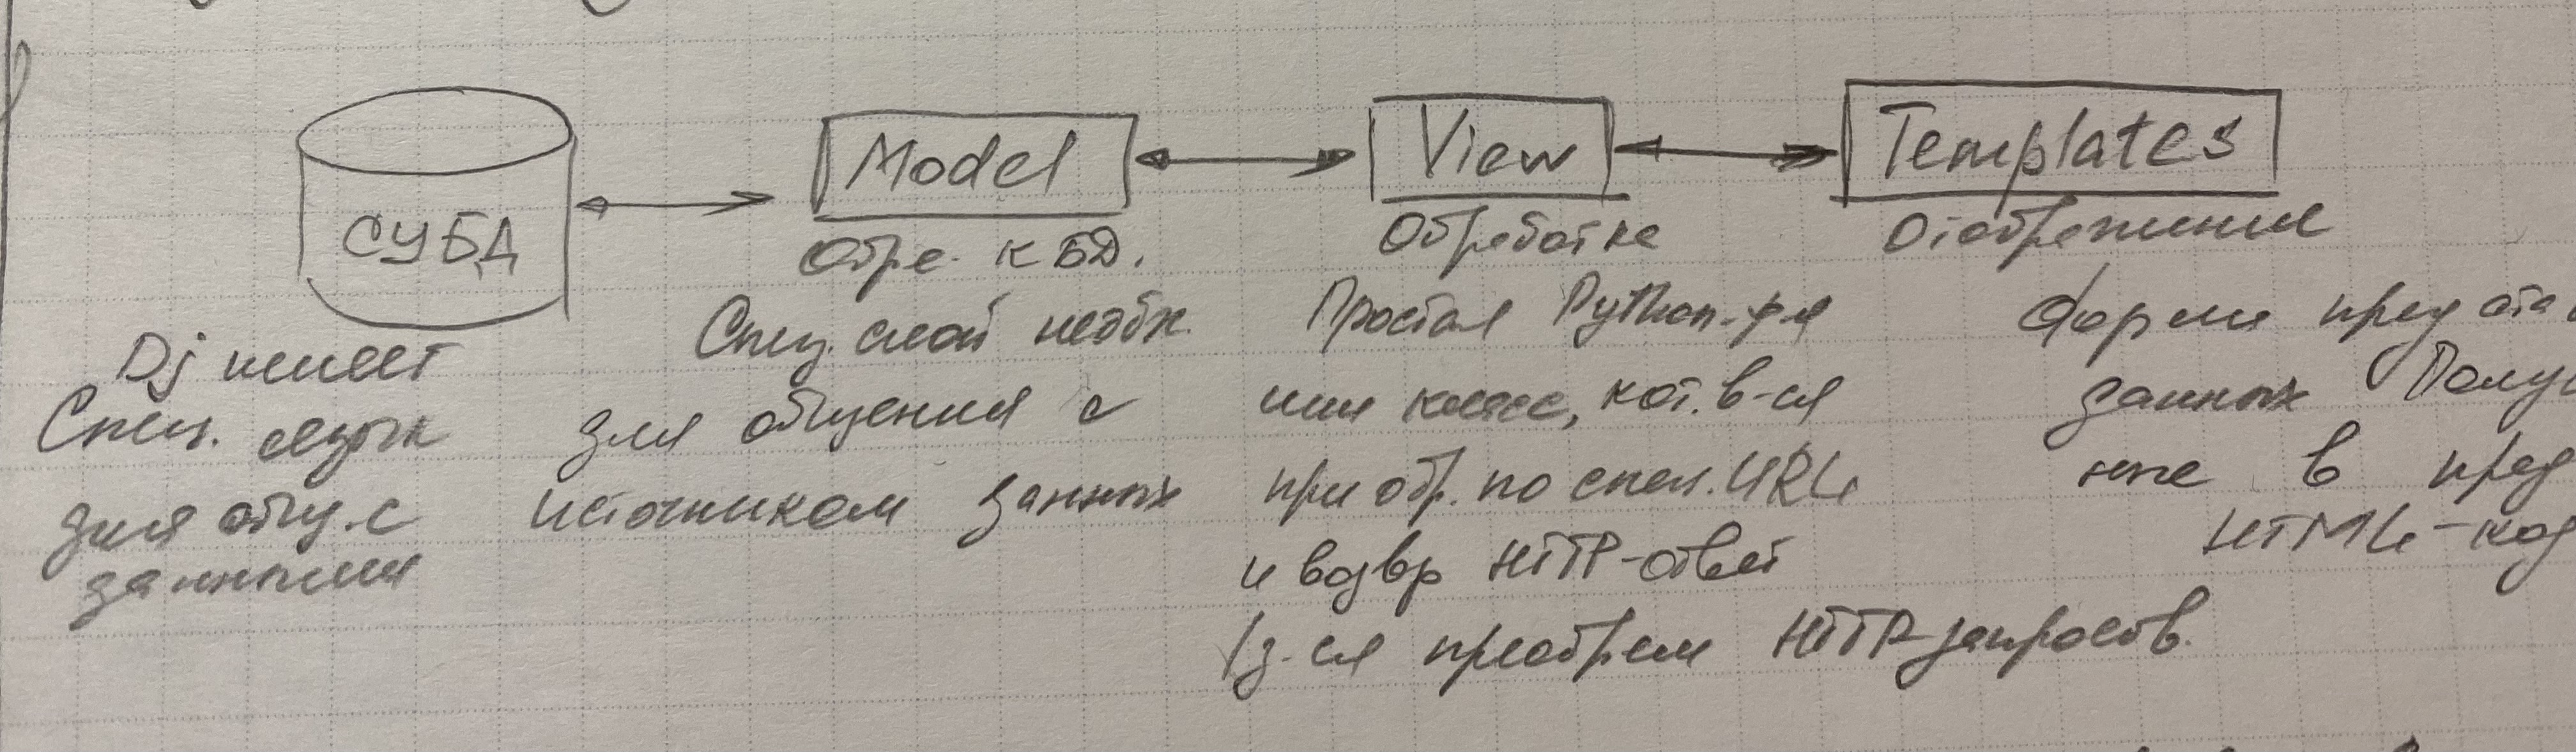
\includegraphics[scale=0.1]{figures/MTV.jpg}
	\caption{MTV}\label{fig:MTV}
\end{figure}



MTV (\ref{fig:MTV}) - model, template, view. Model - специальный слой необходимый для общения с источником данных. Dj имеет специальный язык для общения с данными. View - простая Python функция или класс, который при обращении по спец-URL возвращает HTTP-ответ(занимается преобразование  HTTP-запросов). Templates - отображение, форма представления данных. Получает данные преобразованные в представлении и возвращает HTML-код.

Установка приложения: django-admin startproject todo. Создает каркас и все файлы для работы приложения.

Создание нового приложения:django-admin startapp tasks. Команда вызывается из-под дерриктории проекта.

Миграция данных в БД: python manage.py migrate. В процессе выполнения этой команды создается админка со всеми полями.

Создание пользователя для доступа в приложение: python manage.py createsuperuser. Вводится username, необязательный email-адрес и пароль.

Запуск тестового сервера: python manage.py runserver.

Код обрабатывающий запрос находится в файле  view.py. Если хотим менять отображение, то меняем код именно там.


\textbf{Вопросы:}

1. Что такое HTTP-протокол? Хабр статья "Простым языком об HTTP".

2. Что значит фраза "веб-приложение и веб-фреймворк понятия тождественные но не равные"?

3. Какие еще бывают типы запросов креме GET и POST?

4. Какие еще бывают парамеры(заголовки) запросов?

5. Архитектура Django.

6. Что такое MTV?

7. Что за специальный язык для общения с данными?

8. Какие еще бывают фреймворки для создания веб-приложений?

9. Что такое ORM?

\subsubsection{Что такое HTTP-протокол?}

\subsubsection{Что значит фраза "веб-приложение и веб-фреймворк понятия тождественные но не равные"?}

\subsubsection{Какие еще бывают типы запросов креме GET и POST?}

\subsubsection{Какие еще бывают парамеры(заголовки) запросов?}

\subsubsection{Архитектура Django}

\subsubsection{Что такое MTV?}

\subsubsection{Что за специальный язык для общения с данными?}

\subsubsection{Какие еще бывают фреймворки для создания веб-приложений?}

\subsubsection{Что такое ORM?}

ORM


Создав файл IDLE27.cmd со следующим содержимым:
\begin{lstlisting}[
language = cmd,
numbers = none
]
@echo off
start C:\Python27\pythonw.exe C:\Python27\Lib\idlelib\idle.pyw
\end{lstlisting}


С помощью двойного щелчка по этому файлу можно запустить редактор IDLE для версии Python отличной от версии используемой по умолчанию.




\cite[стр.~34]{chacon:2020}


Пример подстрочной ссылки\footnote{Примечание}






% Источники в "Газовой промышленности" нумеруются по мере упоминания 
\begin{thebibliography}{99}\addcontentsline{toc}{section}{Список литературы}
	\bibitem{chacon:2020}{ \emph{Чакон С.}, \emph{Штрауб Б.} Git для профессионального программиста. -- СПб.: Питер, 2020. -- 496~с. }
	
	\bibitem{sobel:2011}{ \emph{Собель М}. Linux. Администрирование и системное программирование. 2-е изд. -- СПб.: Питер, 2011. -- 880 с. }
\end{thebibliography}

%\listoffigures\addcontentsline{toc}{section}{Список иллюстраций}

\end{document}
